\documentclass[12pt, a4paper]{article}
\usepackage{ctex}
\usepackage{amsmath,amscd,amsbsy,amssymb,latexsym,url,bm,amsthm}
\usepackage{caption}
\usepackage{epsfig,graphicx,subfigure}
\usepackage{enumitem,balance}
\usepackage{wrapfig}
\usepackage{listings}
\usepackage{mathrsfs,euscript}
\usepackage[usenames]{xcolor}
\usepackage{hyperref}
\usepackage[vlined,ruled,linesnumbered]{algorithm2e}
\hypersetup{colorlinks=true,linkcolor=black}

\captionsetup[figure]{
	labelfont = {bf},
	labelformat = {default},
	labelsep = period,
	name = {Fig.}
}

\captionsetup[table]{
	labelfont = {bf},
	labelformat = {default},
	labelsep = period,
	name = {Tab.}
}

\newtheorem{theorem}{Theorem}
\newtheorem{lemma}[theorem]{Lemma}
\newtheorem{proposition}[theorem]{Proposition}
\newtheorem{corollary}[theorem]{Corollary}
\newtheorem{exercise}{Exercise}
\newtheorem*{solution}{Solution}
\newtheorem{definition}{Definition}
\theoremstyle{definition}
\lstset{
	keywordstyle = \color{blue!70}\bfseries, 
	basicstyle = \ttfamily, 
	commentstyle = \ttfamily,
	showstringspaces = false,
	frame = shadowbox,
	rulesepcolor = \color{red!20!green!20!blue!20},
}

\renewcommand{\thefootnote}{\fnsymbol{footnote}}

\newcommand{\postscript}[2]{
	\setlength{\epsfxsize}{#2\hsize}
  	\centerline{\epsfbox{#1}}
}

\renewcommand{\baselinestretch}{1.0}

\setlength{\oddsidemargin}{-0.35in}
\setlength{\evensidemargin}{-0.35in}
\setlength{\topmargin}{-0.3in}
\setlength{\headheight}{0in}
\setlength{\headsep}{0in}
\setlength{\textheight}{10.2in}
\setlength{\textwidth}{7in}
\makeatletter 
\renewenvironment{proof}[1][Proof] {\par\pushQED{\qed}\normalfont\topsep6\p@\@plus6\p@\relax\trivlist\item[\hskip\labelsep\bfseries#1\@addpunct{.}]\ignorespaces}{\popQED\endtrivlist\@endpefalse} \makeatother
\makeatletter
\renewenvironment{solution}[1][Solution] {\par\pushQED{\qed}\normalfont\topsep6\p@\@plus6\p@\relax\trivlist\item[\hskip\labelsep\bfseries#1\@addpunct{.}]\ignorespaces}{\popQED\endtrivlist\@endpefalse} \makeatother

\begin{document}
\noindent

%========================================================================
\noindent\framebox[\linewidth]{\shortstack[c]{
\Large{\textbf{Lab \#3: Community Detection in Networks}}\vspace{1mm}\\
EE447 Mobile Network, Luoyi Fu, Spring 2021\\
\textbf{Due}: \textit{Sunday, May 23rd}}}
\begin{center}

Name: Hongjie Fang  \quad Student ID:518030910150 \quad Email: \href{mailto:galaxies@sjtu.edu.cn}{galaxies@sjtu.edu.cn}
\end{center}

\section{Purpose and Objective}\label{section1}

Modern networks are growing exponentially in size, diversity and complexity. Due to the changes in networks, a wide variety of networks are emerging, such as IoT data, wireless sensor data, cloud data, co-citation in academic fields, and social network data. A community in a network is composed of a set of nodes that are highly connected to each other, unlike other nodes in the network that have relatively random and scattered relationships. A key role of community detection algorithms is that they can be used to extract useful information from the network.

This Lab focuses on the community detection algorithms for network. In this lab, you will use python to complete the community detection under a specific network and visualize the network based on the results. You need to find dataset on the Internet by yourself, use any community detection algorithm to detect the community, and visualize the network based on the community detection results. After programming, you need to answer two questions listed as follows.

\begin{enumerate}
	\item Briefly describe the principle of the community detection algorithm you use.
	\item In addition to visualization, what other applications does the community detection algorithm have? Please list at least three.
\end{enumerate}

\section{Algorithms}
I implement two network detection algorithms in this lab, namely Louvain Algorithm\footnotemark[1] and Leiden Algorithm\footnotemark[2]. They are all based on the notion of modularity. In this section, I will first briefly introduce the definition and meaning of modularity, then introduce two algorithms in details.

\footnotetext[1]{Blondel, Vincent D., et al. "Fast unfolding of communities in large networks." Journal of statistical mechanics: theory and experiment 2008.10 (2008): P10008.}
\footnotetext[2]{Traag, Vincent A., Ludo Waltman, and Nees Jan Van Eck. "From Louvain to Leiden: guaranteeing well-connected communities." Scientific reports 9.1 (2019): 1-12.}
\subsection{Modularity: the Key to the Community}

The notion of modularity\footnotemark[3] is first introduced in the field of physics, and is first brought into the community detection area by Louvain algorithm\footnotemark[1]. The modularity is used to measure whether the division of a community is relatively good result, which has a high similarity of nodes inside the community and a low similarity of nodes outside the community. The formal definition of modularity $Q$ is shown as follows.

$$
Q = \frac{1}{m} \sum_{i,j} \left[A_{ij} - \frac{k_ik_j}{2m}\right]\delta(c_i, c_j)
$$

where $A_{ij}$ is an element of the adjacency matrix of the network, $c_i, c_j$ denotes the two communities where node $i$ and node $j$ are located respectively, and $m$ is the total number of edges in the network, $k_i$ denotes the degree of node $i$. If node $i$ and node $j$ are in the same community, $\delta(c_i, c_j)$ is $1$, otherwise $\delta(c_i,c_j)$ is $0$.

\footnotetext[3]{Newman, Mark EJ. "Analysis of weighted networks." Physical review E 70.5 (2004): 056131.}

In community detection, modularity is regarded as an objective function to optimize. However, the exact modularity optimization is a problem that is computationally hard\footnotemark[3]. As a result, approximation algorithms are necessary for modularity optimization, which leads to many modularity-based community detection algorithm. Therefore, we say that modularity is the ``key'' to the community.

\subsection{Louvain Algorithm}

The main idea of Louvain algorithm can be summarize as ``\textbf{greedily combine the node with the community of its neighbors in order to increase modularity, then reconstruct the graph according to the community, and repeat the process until modularity converges}''.

In short, the procedure of Louvain algorithm can be listed as follows.

\begin{enumerate}
	\item[\textbf{Step 1}.] Check every node in the graph in a random order, and determine whether combine it with the community of one of its neighbor may increase the modularity. If so, combine the current node with the community which can receive the biggest modularity gain.
	\item[\textbf{Step 2}.] Repeat Step 1 until no modularity gain is available. Then go to Step 3. 
	\item[\textbf{Step 3}.] Reconstruct the graph and combine all nodes in a community into one node representing for the community, and the edge between nodes becomes the edge between communities (which may result in self-loop, and it is a valid situation).
	\item[\textbf{Step 4}.] Go back to Step 1 and repeat Step 1 to Step 3, until the reconstructed graph is same as the given graph, \textit{i.e.}, no modularity gain is available under the current circumstances. 
\end{enumerate}

An example\footnotemark[1] of the procedure of Louvain algorithm is illustrated in Fig. \ref{fig1} as follows.

\begin{figure}[htbp]
	\centering
	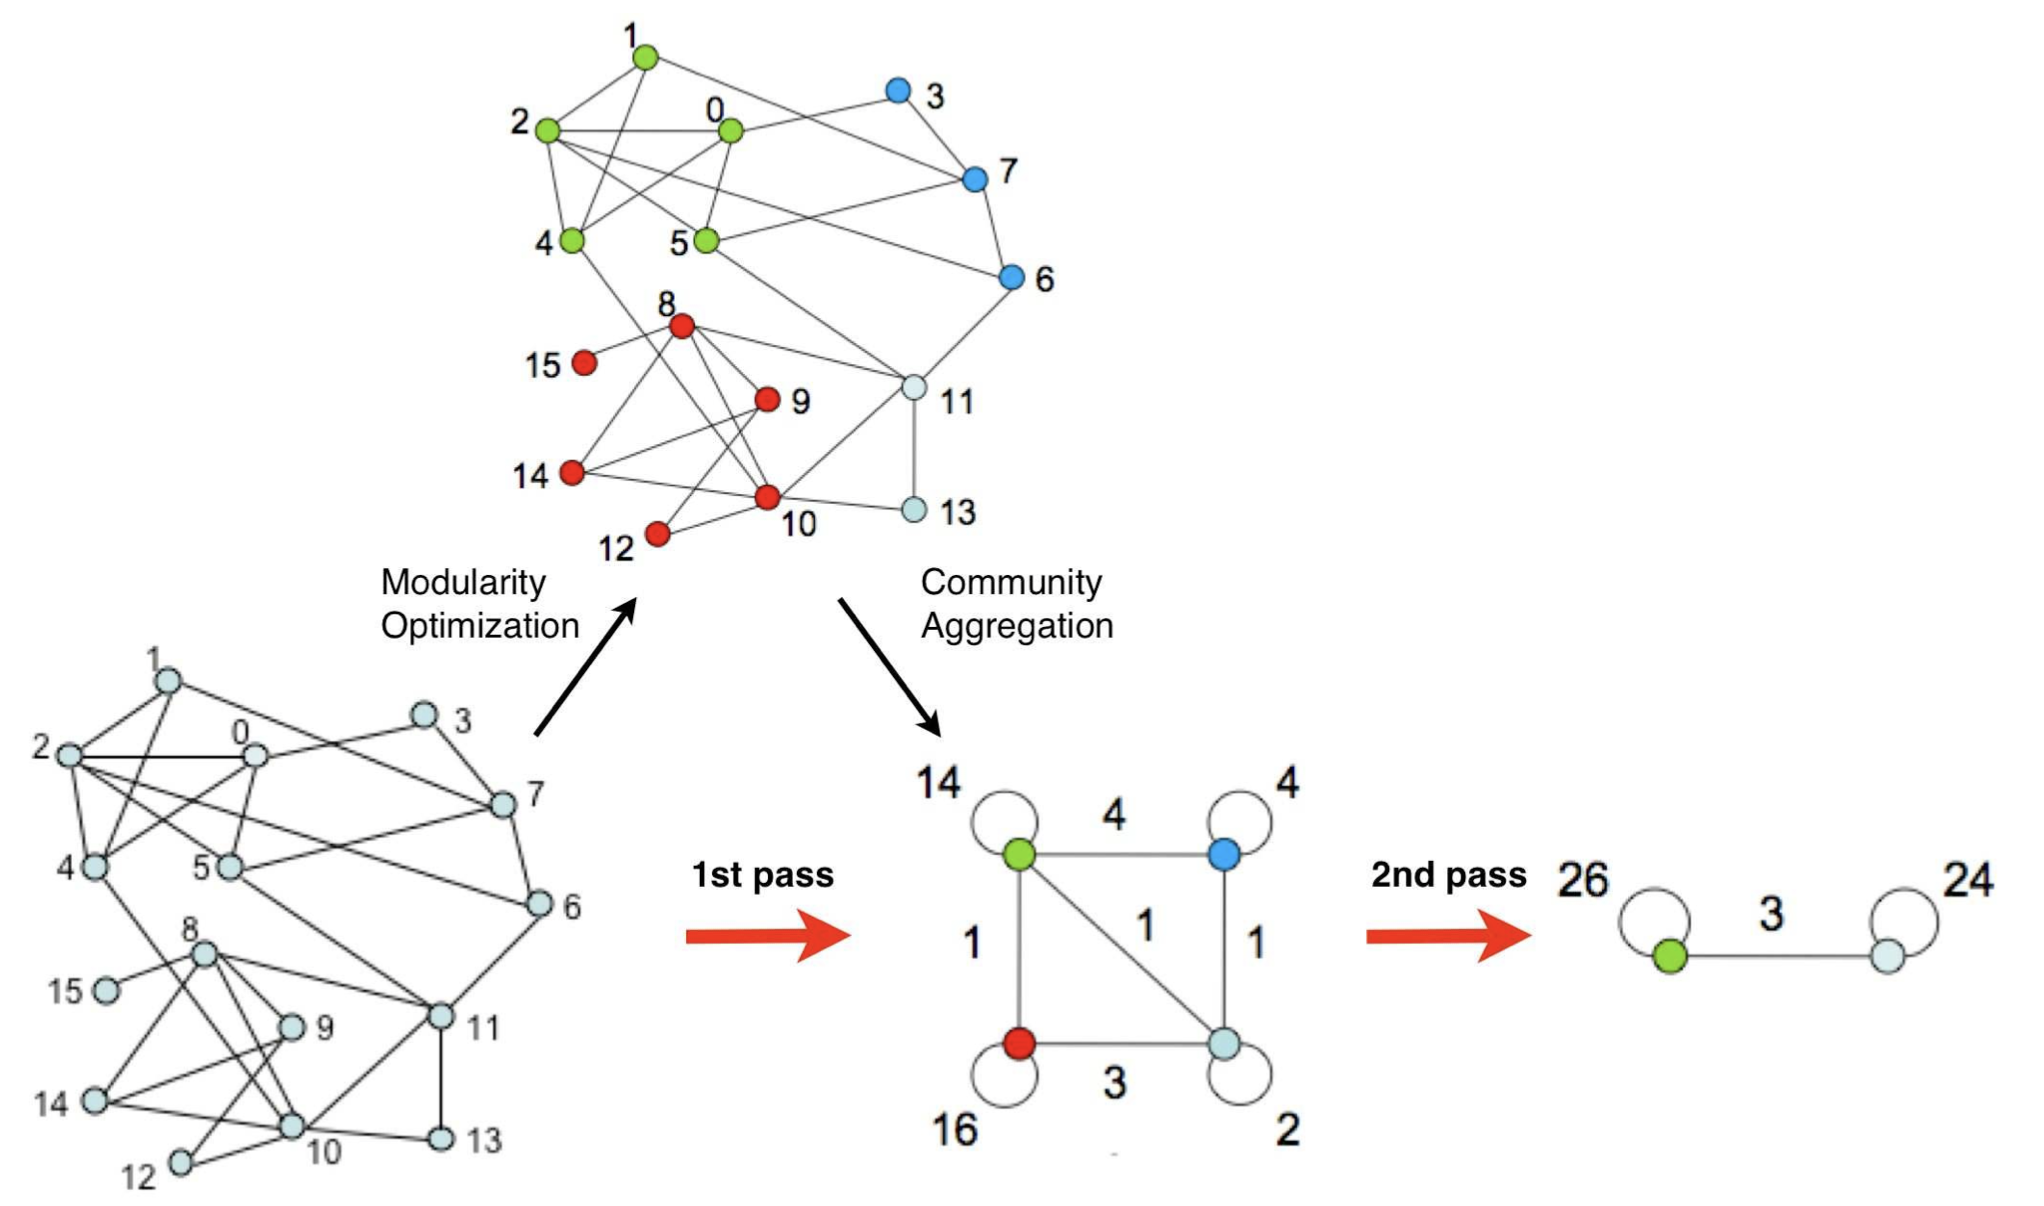
\includegraphics[width=4.5in]{1.png}
	\caption{An example of Louvain algorithm}
	\label{fig1}
\end{figure}

\footnotetext[1]{Blondel, Vincent D., et al. "Fast unfolding of communities in large networks." Journal of statistical mechanics: theory and experiment 2008.10 (2008): P10008.}
\footnotetext[3]{Newman, Mark EJ. "Analysis of weighted networks." Physical review E 70.5 (2004): 056131.}

\subsection{Leiden Algorithm}
Leiden algorithm is an improvement of Louvain algorithm. Notice that Louvain algorithm may produce badly-connected communities, that is, a community may be disconnected if we only focus on edges inside the community, which is caused by the graph reconstruction process. The Leiden algorithm states that \textbf{we cannot reconstruct the graph directly according to the their community, but reconstruct the graph by only combine those well-connected subset of communities}. The combination process is simply a copy of the first step of node merging, except that we only merge nodes within the same community and disallow the bad-connected nodes to be merged together. Besides, the Leiden algorithm also use the idea of breadth-first search to optimize the first step of node merging.

In short, the procedure of Leiden algorithm can be listed as follows.

\begin{enumerate}
	\item[\textbf{Step 1}.] Initialized a queue with every node in the graph in a random order. For every iteration, fetch a node from the queue and determine whether combine it with the community of one of its neighbor may increase the modularity. If so, combine the current node with the community which can receive the biggest modularity gain. Then, push the neighbor of the changed node into the queue, and we only need to examine those nodes because of the locality of the community modifications. Repeat Step 1 until the queue is empty.
	\item[\textbf{Step 2}.] Refine the partition obtained by Step 1 by only considering the nodes in the partition at one time. Intialize the refined partition as a singleton partition, then merge the nodes into the community in the refined partition if the community is well-connected. Repeat the process until no merge is available.
	\item[\textbf{Step 3}.] Reconstruct the graph and combine all nodes in a community into one node representing for the community according to the refine dcommunity, and the edge between nodes becomes the edge between communities (which may result in self-loop, and it is a valid situation).
	\item[\textbf{Step 4}.] Go back to Step 1 and repeat Step 1 to Step 3, until the reconstructed graph is same as the given graph, \textit{i.e.}, no modularity gain is available under the current circumstances. 
\end{enumerate}

An example\footnotemark[2] of the procedure of Leiden algorithm is illustrated in Fig. \ref{fig2} as follows.
\footnotetext[2]{Traag, Vincent A., Ludo Waltman, and Nees Jan Van Eck. "From Louvain to Leiden: guaranteeing well-connected communities." Scientific reports 9.1 (2019): 1-12.}

\begin{figure}[htbp]
	\centering
	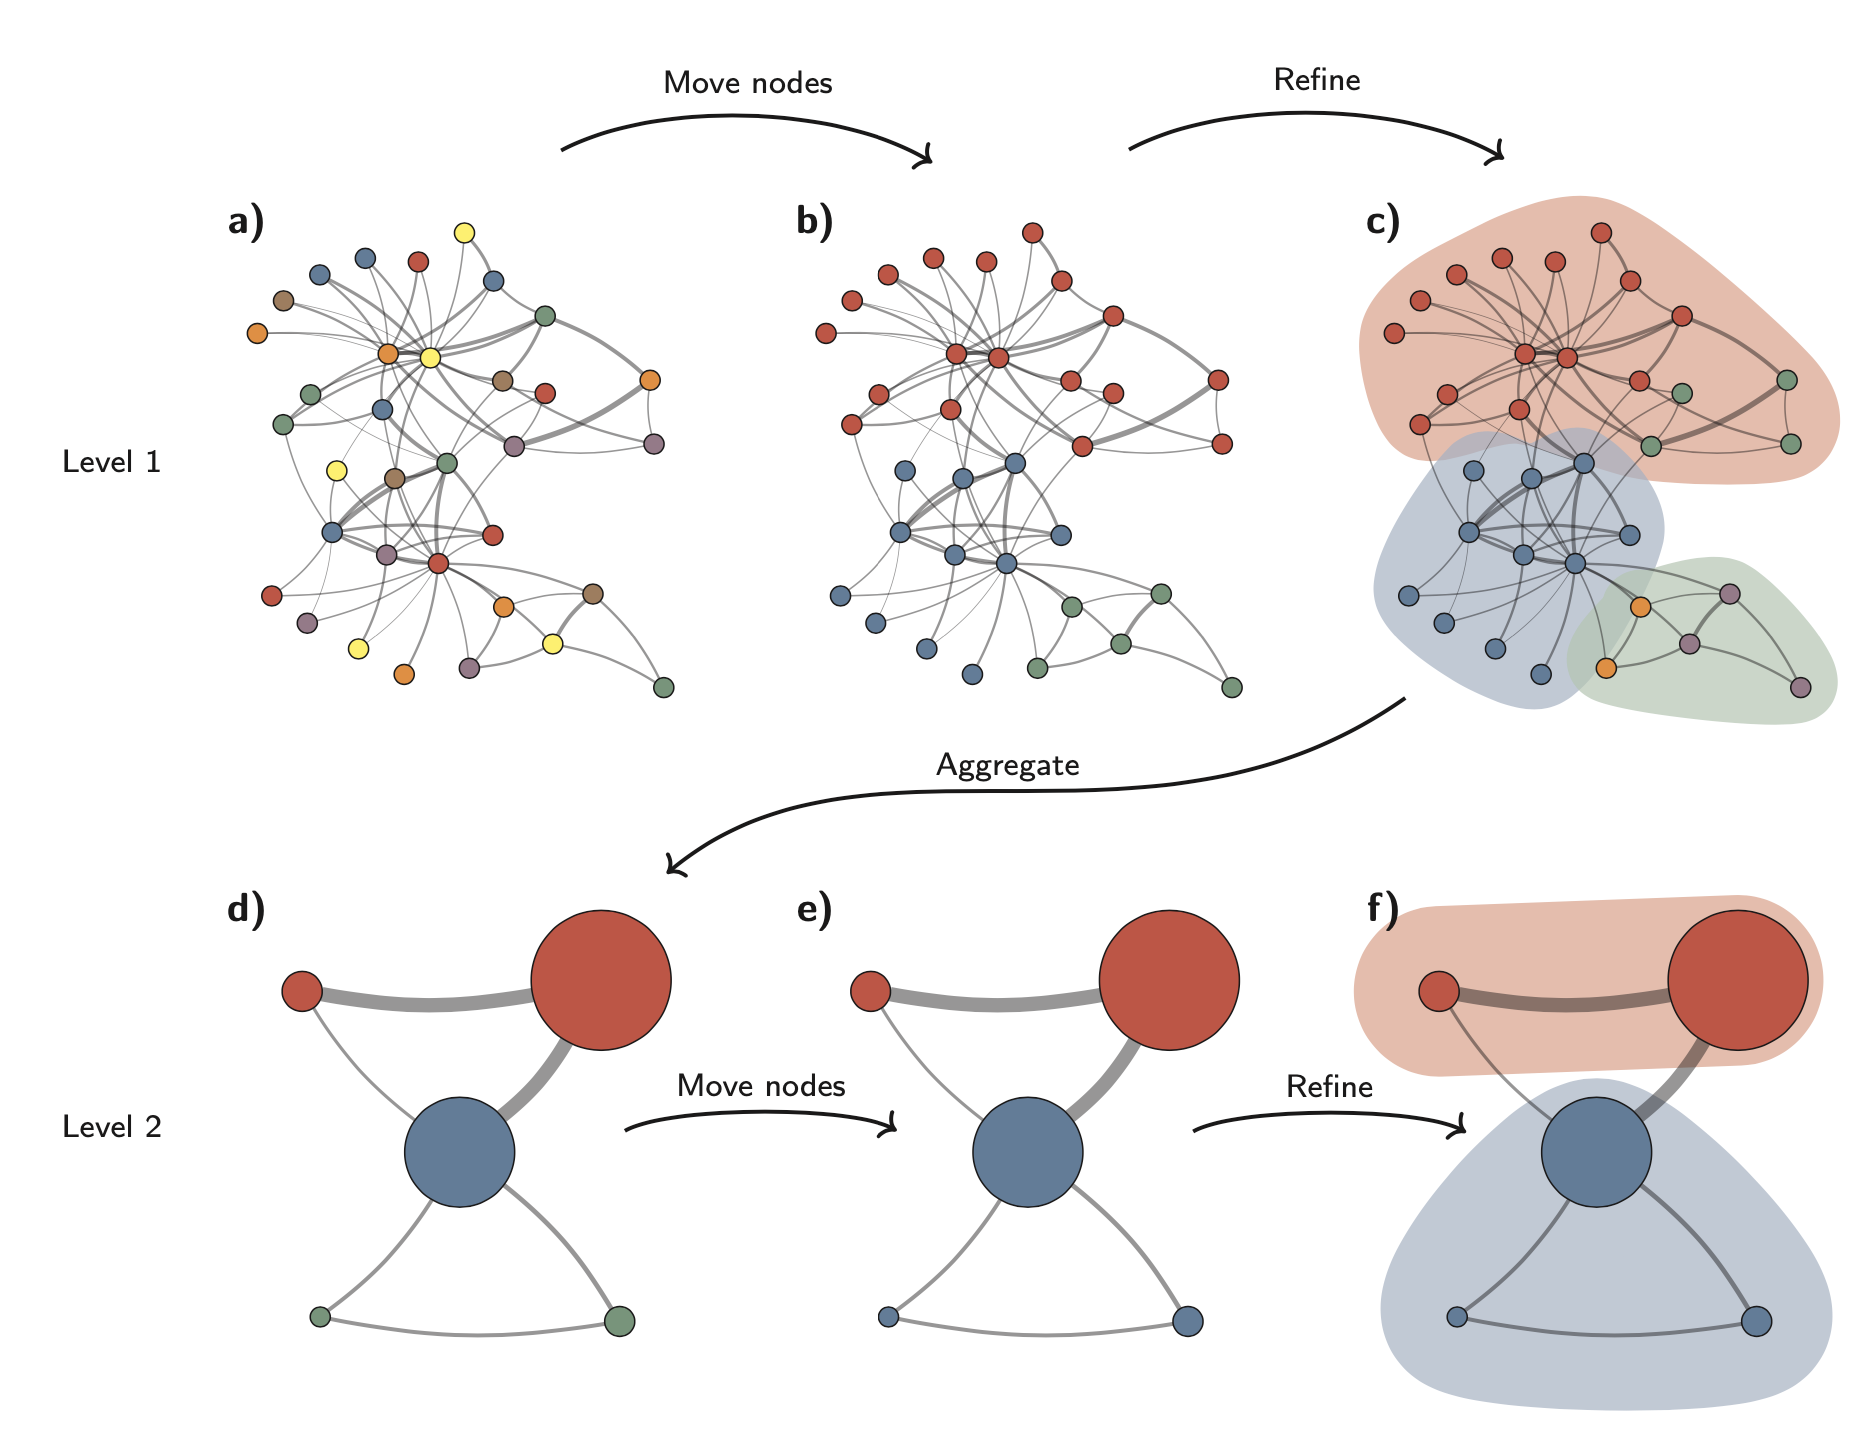
\includegraphics[width=4.7in]{2.png}
	\caption{An example of Leiden algorithm}
	\label{fig2}
\end{figure}

\section{Implementations and Experiments}
Notice that I do not use any advanced clustring or community detection API in this lab in order to deepen the understanding of the community detection algorithms mentioned before. I implement the Louvain algorithm and the Leiden algorithm from zero. The process is not so difficult since the algorithms are more about the exquisite thoughts but less about the difficult techniques.

For dataset, I use two datasets, namely the DBLP collabration dataset\footnotemark[4] and the Starwars social network dataset\footnotemark[5]. The first dataset is relatively large, which is used to test the speed and performance of two community detection algorithms. The second dataset is relatively small, which is used to visualize the results of the community detection in an intuitive way.

\footnotetext[4]{J. Yang and J. Leskovec. Defining and Evaluating Network Communities based on Ground-truth. ICDM, 2012}
\footnotetext[5]{\url{https://www.kaggle.com/ruchi798/star-wars}}

\subsection{Speed and Performance: DBLP Collabration Dataset}
The Leiden algorithm claims that it runs up to 20x faster than the Louvain algorithm, and it produces less bad-connected communities. Unfortunately, the quality of the community detection CANNOT only be determined by the modularity, and high modularity can also produces bad-connected communities. Therefore, Leiden algorithm may produce results with lower modularity but higher quality. We now test the speed and performance of two algorithms on the DBLP Collabration dataset, since it has more than 300, 000 nodes and more than 1,000,000 edges, which is a relatively great benchmark to test the speed and performance of a community detection algorithm.

Now, we list the quantitative results in Tab. \ref{tab:expr-speed-1} as follows.

\begin{table}[htbp]
    \centering
    \begin{tabular}{ccccccc}
        \hline 
        Algorithms & Epoch 1 & Epoch 2 &  Epoch 3 & Epoch 4 & Epoch 5 & Total Time \\
        \hline
        Louvain & 200.84 & 92.32 & \textbf{37.13} & \textbf{6.58} & \textbf{1.07} & 337.94 \\
		Leiden & \textbf{143.71} & \textbf{77.51} & 62.13 & 32.43 & 13.36 & \textbf{329.14}\\
        \hline
    \end{tabular}
    \caption{The speed of Louvain algorithm and Leiden algorithm in each epoch (unit: second)}
    \label{tab:expr-speed-1}
\end{table}

From Tab. \ref{tab:expr-speed-1}, we can see that in the first two epochs, the Leiden algorithms is obviously faster than Louvain algorithm, but in the next few epochs, Leiden algorithm is slower than Louvain algorithm. It is because that the Leiden algorithm does not reconstruct the graph thoroughly, and in the next epochs, the size of the induced graphs in Louvain algorithm and Leiden algorithm may have a huge difference, resulting in the speed difference. At least in the first epoch, the size of the graph is same in two algorithms, so according to the experimental results on DBLP collabration dataset, we can conclude that when the size of the graph is fixed, Leiden algorithm is faster than Louvain algorithm.

The Louvain algorithm gives a community partitioning result of modularity about $82.14$, and the Leiden algorithm gives a community partitioning result of modularity about $68.07$. The reason of the modularity difference is already explained in the first paragraph. According to the number of communities in the partition, the Leiden algorithm produces about 5 times more communities than the Louvain algorithm, which implies that Leiden algorithm produces less bad-connected communities indirectly.

In all, \textbf{the Leiden algorithm is faster than the Louvain algorithm}, and \textbf{the Leiden algorithm has lower modularity score, but produces less bad-connected communities}.

\subsection{Visualization: the Starwars Social Network Dataset}

We use Louvain algorithm and Leiden algorithm to find the communities in the Starwars social network dataset, and the results are illustrated as follows.

\begin{figure}[htbp]
	\centering
	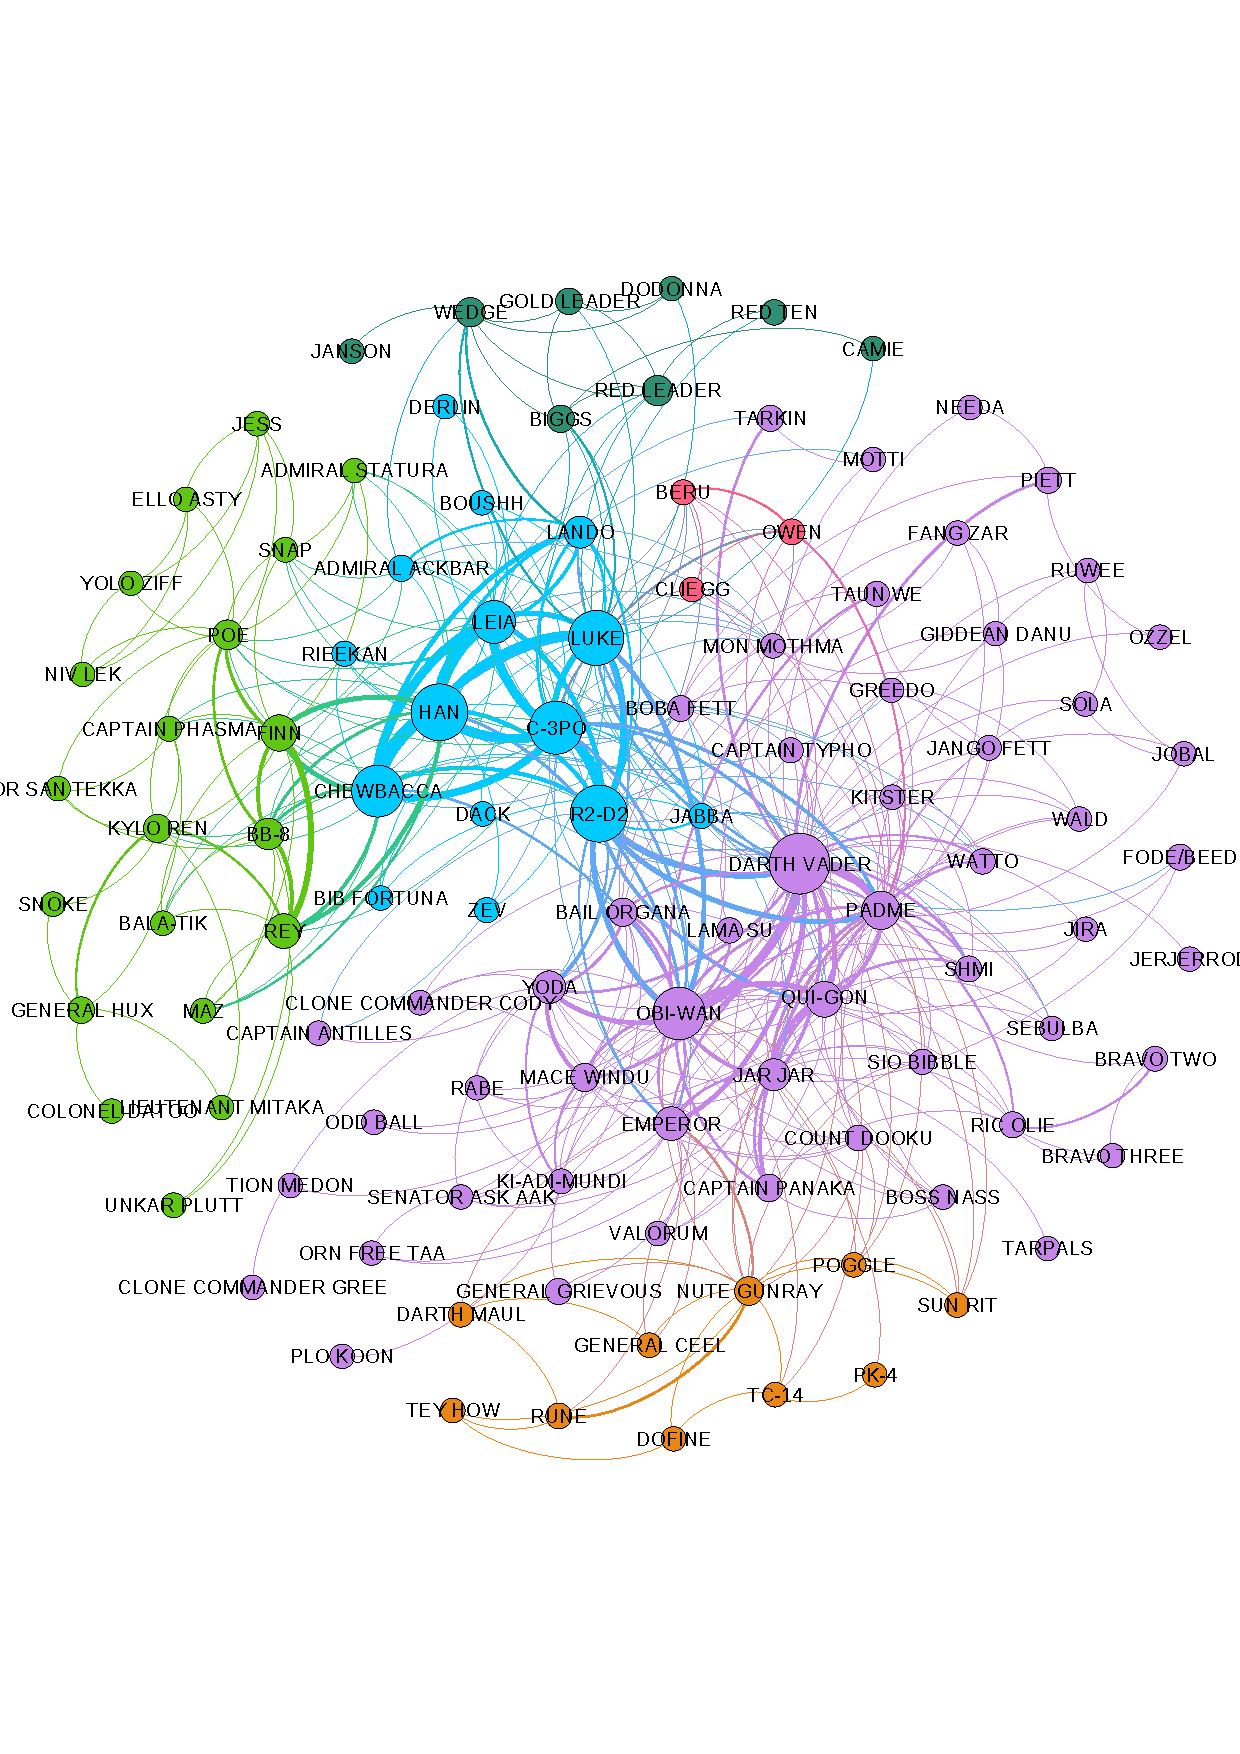
\includegraphics[width=0.9\textwidth]{3.pdf}
	\caption{The visualization result of the community detection results of Louvain algorithm on Starwars social network dataset, where different colors indicates different communities}
	\label{fig3}
\end{figure}

\begin{figure}[htbp]
	\centering
	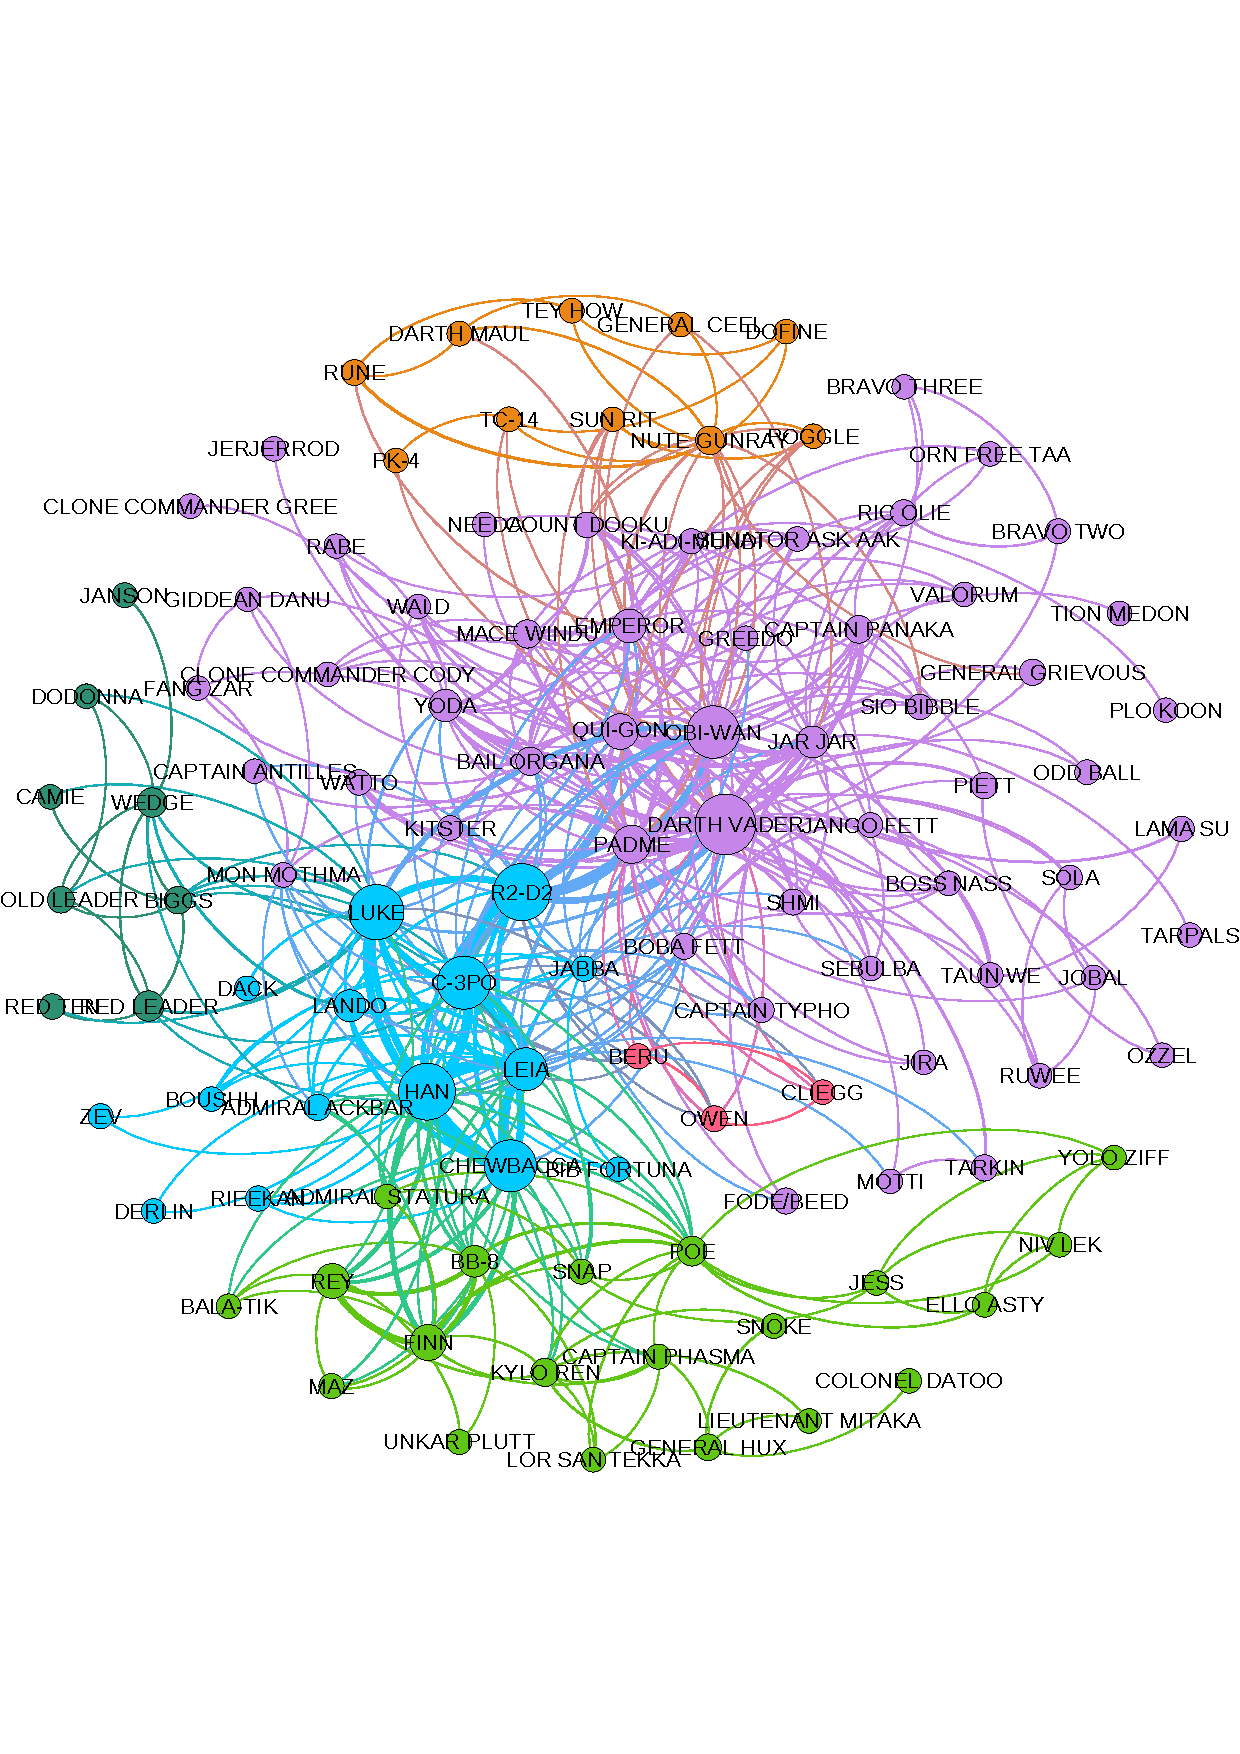
\includegraphics[width=0.9\textwidth]{4.pdf}
	\caption{The visualization result of the community detection results of Leiden algorithm on Starwars social network dataset, where different colors indicates different communities}
	\label{fig4}
\end{figure}

From Fig. \ref{fig3} and Fig. \ref{fig4} we can observe that both Louvain algorithm and Leiden algorithm performs well on small datasets. According to the knowledge of Starwars series movies, we can see that both algorithms have recognized the Galatic Empire community (the purple colored communities in both figures), and the Rebel Alliance (the blue colored communities in both figures). Therefore, we can conclude that both algorithms can find out communities and achieve a high accuracy.

\section{Further Discussions}
In this section, we will answer the questions mentioned in the first section.

\begin{enumerate}
\item \textbf{Q}: Briefly describe the principle of the community detection algorithm you use.
      
\textbf{A}: Both Louvain algorithm and Leiden algorithm is based on the principle that \textbf{greedily merge the nodes into the community of its neighbors to increase modularity}. But instead of only focusing on the modularity, Leiden algorithm also considers the problem of bad-connected communities, and use refined graph to improve the quality of partition.
\item \textbf{Q}: In addition to visualization, what other applications does the community detection algorithm have? Please list at least three.

\textbf{A}: Other applications of community detection includes:
\begin{itemize}
\item \textbf{Customized Recommendations} (Smart Advertising and Targeted Marketing): find the communities in the user group, and use other users' habits to make recommendations to the user in the same community.
\item \textbf{Link Prediction}: use community detection results to predict whether there is a link between two nodes. If two nodes are in the same community, then the probability that there is an edge between them is a little bit higher. Therefore, the community detection algorithms can be used as an auxiliary approach to link prediction.
\item \textbf{Network Privacy}: Community detection provides a group-level point of view of a network, and it can also be used to break privacy of people on weak signal networks like Bitcoins, which leads to some applications in the weak signal networks to extract the privacy of users.
\item \textbf{Criminology}\footnotemark[6]: use community detection to find out the criminal groups and prevent further criminal activities.
\item \textbf{Politics}\footnotemark[6]: politicians can use the community detection results to track their supporters and fight for the votes of other peoples in the same community with their supporters.
\end{itemize} 
\end{enumerate}
\footnotetext[6]{Karataş, Arzum, and Serap Şahin. "Application areas of community detection: A review." 2018 International congress on big data, deep learning and fighting cyber terrorism (IBIGDELFT). Ieee, 2018.}


\section{Conclusion}

In this lab, we dive deeply into the community detection algorithms. I implement two famous modularity-based algorithms by myself, namely the Louvain algorithm and the Leiden algorithm. Their ideas are quite simple: try to optimize the modularity by greedily merge singleton nodes into its neighborhood communities. Such simple idea may lead to satisfactory results illustrated before, which suprised me and make me to think that the simplicity of the algorithm is also an important view to judge the quality of an algorithm. The algorithms also inspires me to develop more simple but efficient algorithms in the further researches.

In order to finish the lab, I read many papers about community detection, and gain a lot of knowledge about the community detection fields, which helps me a lot in the data mining area. Also, in order to completes visualization, I learnt to use Gephi\footnotemark[7] to visualize the network in a more intuitive way, which also benifits me in the further researches.

\footnotetext[7]{\url{https://gephi.org/}}

The full implementation codes of the lab is available in my \href{https://github.com/Galaxies99/EE447-CourseData/tree/main/Labs/Lab3}{github repository}, or you can see the attached files for details. To execute the code, just enter the \texttt{community} folder and execute one of the followings:

\begin{lstlisting}[language=bash]
python louvain_dblp.py
python leiden_dblp.py
python louvain_starwars.py
python leiden_starwars.py
\end{lstlisting}

The four lines correspond to the two algorithms on two different datasets introduced before. For other questions about the source code, please feel free to send an e-mail\footnotemark[8] to me.

\footnotetext[8]{\url{mailto:galaxies@sjtu.edu.cn}}
%========================================================================
\end{document}
